\documentclass{article}
\usepackage{ShumanNotes}
\title{Homework 1: Welcome to ECE 111}
\author{Derek Gorton}
\date{Due October 4th @ 3 PM, 2012}
\setlength{\parindent}{0pt}
\pdfpagewidth 8.5in
\pdfpageheight 11in

\begin{document} 
\maketitle

\section{Introduction}
Welcome to ECE 111 my name is Matt Shuman and I lived in Madras, Oregon before coming to OSU for undergraduate studies in Fall 2001, and now Corvallis is home.  I am teaching three ECE courses (ECE 111, 271, and 507), taking three MBA courses (BA560\footnote{http://mime.oregonstate.edu/research/drl/}, 562, and 528), and teaching a woodworking class at the OSU craft center\footnote{http://mu.oregonstate.edu/craftcenter/}.  It's a busy term, but I'm excited for this term. Insert your image as in figure \ref{golf} using the link below and briefly introduce yourself.
\centerimage{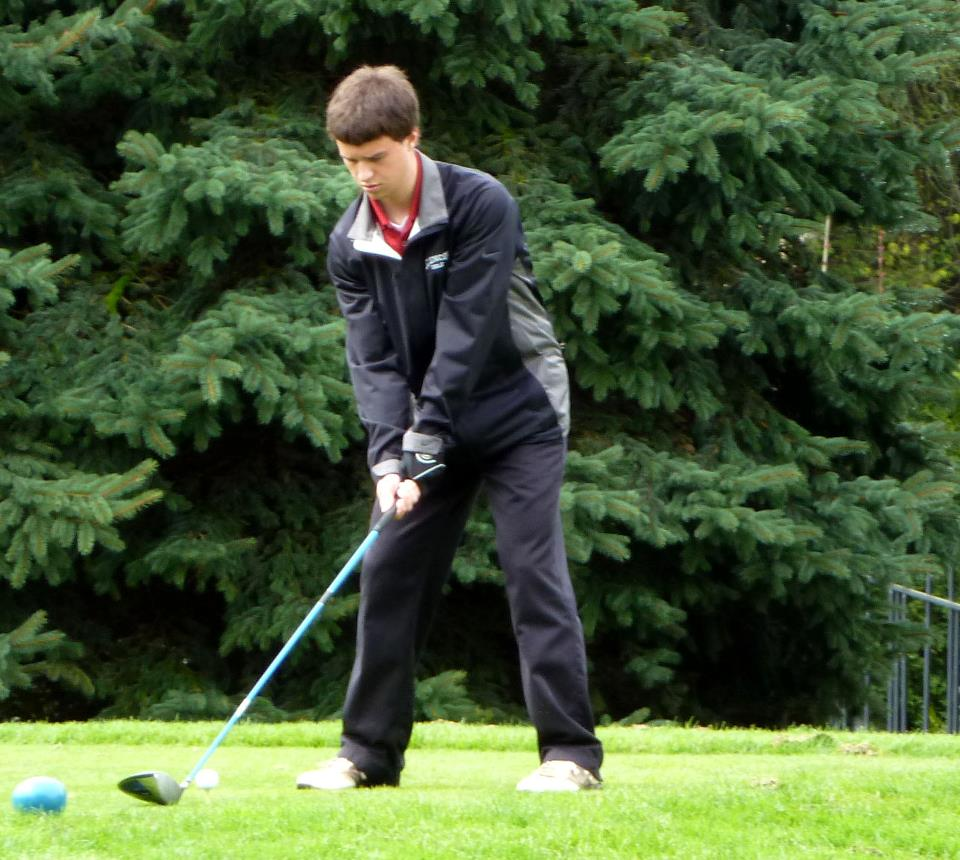
\includegraphics[width = 2in]{./Golf.jpg} }{Me playing golf}{golf}\newline
\newline

my name is Derek Gorton. I lived in corvallis a long time ago then i moved to hillsboro OR. i am really happy to be back in corvallis because i love the college and i love the beavers. I really like to play sports and i played golf in high school. i enjoy solving puzzles like rubiks cubes and learing about how things work. my favorite class is math because i enjoy solving problems and seeing how to get the answers.
.  
\section{Defining Success}
\emph{Success is the achievement of something desired, planned, or attempted. After you put years and thousands of dollars into your 
college education, what do you want from your ECE degree?}
\newline\newline
when i come out of college i want to be able to solve problems with computers. i know that it is going to be hard and its going to take a lot of studying to get through school but i know that i have to work hard today to feel the success tomorrow. when i look at an engineer i see a person who is really smart an can solve problems and thats what i want to be.

\section{Word Processing}
\emph{The homework assignments in ECE 111 focus on using Latex to typecast a professional looking .pdf for each assignment.  What are the advantages of Latex compared to traditional WYSIWYG \footnote{http://en.wikipedia.org/wiki/WYSIWYG} word processors?  What are the disadvantages of using Latex?}\newline\newline

Although Word is a useful and practical tool for writing short and simple documents, it becomes too complex or even unusable when one wants the word processor to do more complicated tasks. Many rather commonly needed features, like user-customised automated numbering or various automated indexes. LaTeX does require more effort and time to learn to use even for simpler tasks, but once learned, difficult tasks can be accomplished rather easily.
 \newline 
\section{Microcontrollers}
Atmel Microcontrollers are a very inexpensive way to develop projects.  Every future project in ECE 111 will use an Atmel Microcontroller, the Atmel Tiny26.\newline
\emph{Lookup the cost of the Tiny26 Microcontroller from Digikey}\newline
\url{http://search.digikey.com/scripts/DkSearch/dksus.dll?Detail&name=ATTINY26L-8PU-ND}.
\newline \newline
\emph{3.06 dollars}\newline






\section{Microcontroller Packages}
Integrated Circuits, ICs, are made using many different types of packages. The Tiny26 in lab is a DIP , while the 5 volt regulator is in a TO-92 package. The ECE 272 CPLD uses a 44 pin QFP. The Droid X OMAP processor is a BGA package type with over 400 pins! \newline
\newline
\emph{Insert a picture for the DIP, TO-92, QFP, and BGA package types}\newline
\newline
This link might be helpful \newline
\newline
\url{http://en.wikipedia.org/wiki/Chip_carrier}\newline
\newline


\picsidebyside{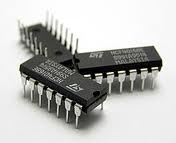
\includegraphics[width=1in]{./dip2.jpg}}{DIP}{name1}{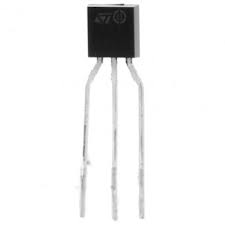
\includegraphics[width=1in]{./92to.jpg}}{TO92}{name2}

\picsidebyside{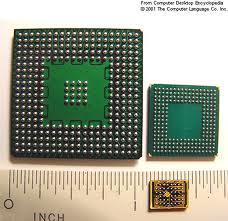
\includegraphics[width=1in]{./BGA2.jpg}}{BGA}{name1}{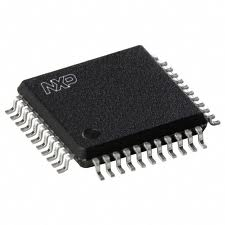
\includegraphics[width=1in]{./QFP2.jpg}}{QFP}{name2} 

\cfoot{ECE 111 Homework \#1}

\end{document}
